\begin{tikzpicture}[x=0.103mm,y=-0.103mm]
  \node[anchor=north west,inner sep=0] at (0,0) {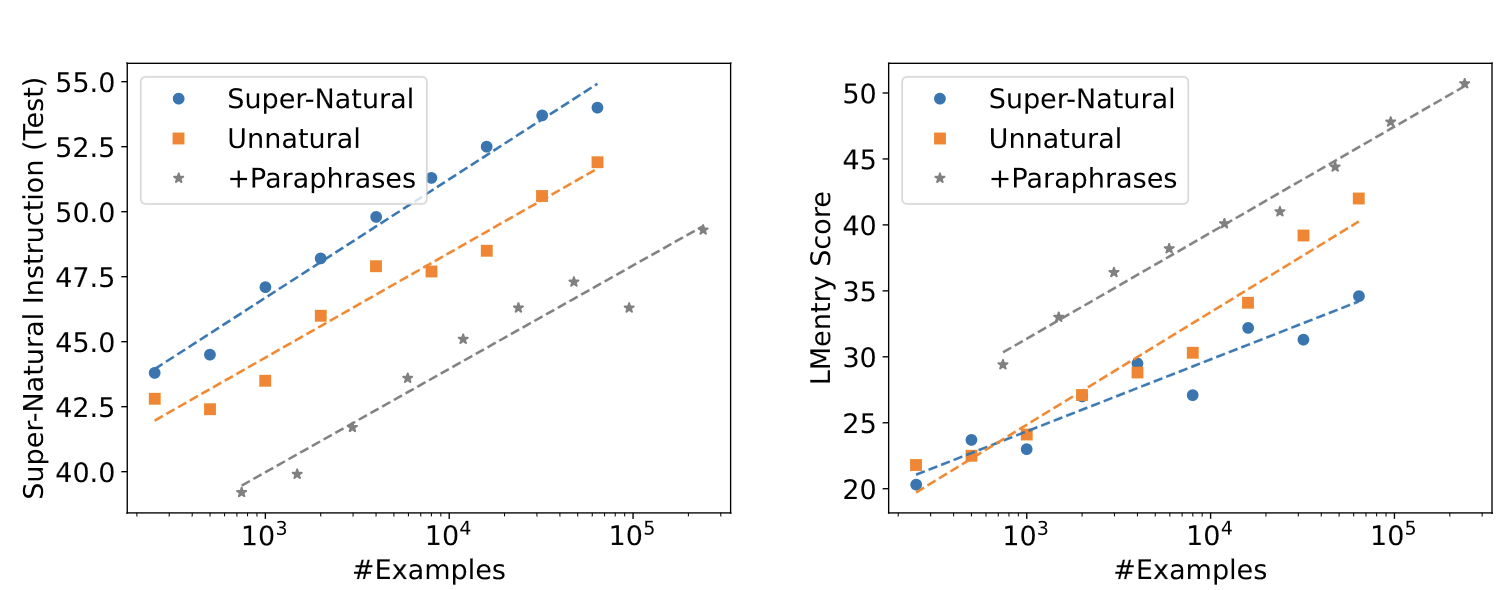
\includegraphics[width=155.118mm]{part6/visuals/unnatural.png}};
  \fill[white] (8,73) rectangle (48,510);
  \node[rotate=90,font=\footnotesize] at (31,291) {Super-Natural Instruction（测试）};
  \fill[white] (797,177) rectangle (839,430);
  \node[rotate=90,font=\footnotesize] at (817,302) {LMentry 得分};
  \fill[white] (217,159) rectangle (421,195);
  \node[anchor=west,font=\footnotesize] at (223,177) {+释义改写};
  \fill[white] (976,158) rectangle (1181,196);
  \node[anchor=west,font=\footnotesize] at (983,177) {+释义改写};
  \fill[white] (337,550) rectangle (529,588);
  \node[font=\footnotesize] at (432,569) {样本数};
  \fill[white] (1097,550) rectangle (1289,588);
  \node[font=\footnotesize] at (1193,569) {样本数};
\end{tikzpicture}
